%!TEX root = foo-thesis.tex

\chapter{Überblick}
\label{chap:overview}

Das Ziel dieser Arbeit ist eine hinreichend genaue und effiziente Erkennung von Straßenschäden in 3D-Punktwolken auf Basis einzelner Punkte. Dazu sollen in diesem Kapitel die Objekte von Interesse sowie die grundlegende Systemumgebung dargestellt werden. Konzepte und Implementierungen hinter den für die Erkennung nötigen Verarbeitungsschritten werden in den folgenden Kapiteln erläutert. Dabei wird sowohl auf den eigens konstruierten Ansatz per \textit{Feature-Extraction} eingegangen als auch auf einen auf \textit{Deep Learning} basierenden.

\section{Maschinelles Lernen}

Das maschinelle Lernen ist ein Teilgebiet der künstlichen Intelligenz und gliedert sich selbst wiederum in viele Zweige. Einer davon ist das \textit{Deep Learning}, das in Kapitel \ref{chap:intro} kurz eingeführt wurde. Ein generell häufig genutztes Paradigma ist das überwachte Lernen, dessen Basis Paare von Eingabe und gewünschter Ausgabe sind \citep{Jung-2020}. Die manuelle Erstellung solcher Paare wird \textit{Annotation} genannt. Mit diesen Informationen werden Modelle trainiert, zum Beispiel \textit{Random Forests} oder \textit{Support Vector Machines}. Das meint den iterativen Prozess einer Vorhersage (nachfolgend \textit{Prediction}) der Ausgabe zu gegebener Eingabe sowie anschließender Verbesserung des Modells anhand der gemachten Fehler. Meist werden Training und \textit{Prediction} nicht direkt auf der Eingabe, sondern auf daraus extrahierten \textit{Features} durchgeführt. Dabei entstehen Featurevektoren, welche die Eingabe kompakt und aussagekräftig repräsentieren sollen, sodass das Modell sinnvolle Schlüsse aus ihnen ziehen kann. \\
Für den in dieser Arbeit behandelten Anwendungsfall der semantischen Segmentierung von Punktwolken sind die einzelnen Punkte die Eingabe, aus denen Features extrahiert werden, und die Klassen die Ausgabe. Dieser grundsätzliche Ablauf des \textit{Feature-Extraction}-Ansatzes mit \textit{Random Forests} als Modell ist in Abbildung \ref{fig:ml_process} illustriert. Erläuterungen zu den einzelnen Schritten werden in den folgenden Kapiteln gegeben. Zum Trainieren des Modells und zum Testen von dessen Qualität werden eine Trainings- sowie Testpunktwolke benötigt. Genauere Daten zu diesen finden sich in Kapitel \ref{chap:eval}, wobei etwaige Bilder von Punktwolken in dieser Arbeit ebenfalls von diesen beiden stammen.

\begin{figure}[!ht]
    \centering
    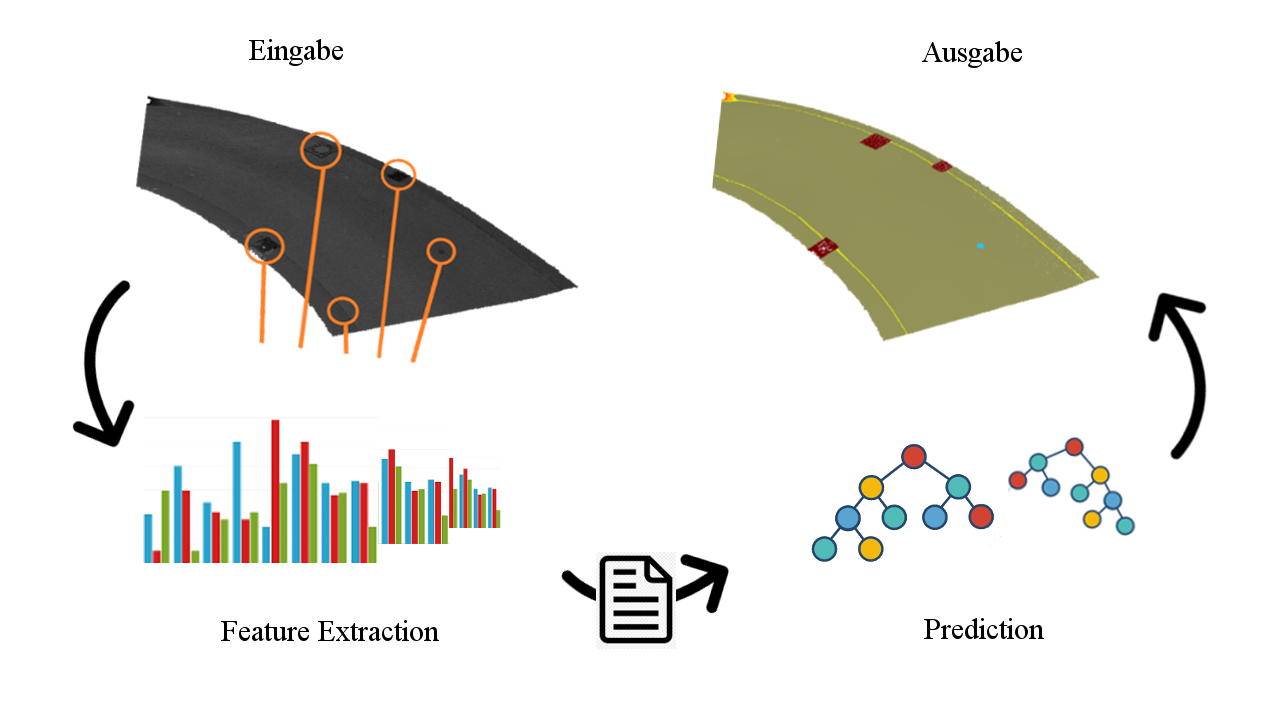
\includegraphics[width=0.95\textwidth]{graphics/ml_process_adv}
    \caption{Ein High-Level-Blick auf den Ablauf des Feature-Extraction-Ansatzes.}
    \label{fig:ml_process}
\end{figure}

\section{Betrachtete Objektklassen}

Entsprechend des Ziels nehmen Objekte, die auf einen mangelhaften Straßenzustand hinweisen, den vornehmlichen Fokus ein. Einfluss auf die Entstehung von Schäden verschiedener Art haben unter anderem der Niederschlag, temperaturbedingte Verformungen sowie die Verkehrsbelastung selbst.\footnote{https://www.ise.kit.edu/rd\_download/SBT/Kolloquium\_SBT\_2011-11-23\_C.Karcher.pdf} Es existieren Leitfäden\footnote{https://itzeb.heller-ig.de/leitfaden/} zur empfohlenen Auswertung solcher \textit{Substanzmerkmale}, an denen sich unter anderem bezüglich der verschiedenen Klassen orientiert wurde. Diese Klassen sind zum besseren Verständnis als Bilder von Punktwolken in Abbildung \ref{fig:all_classes} dargestellt.

\begin{figure}
    \subcaptionbox{unbeschädigte Straße}{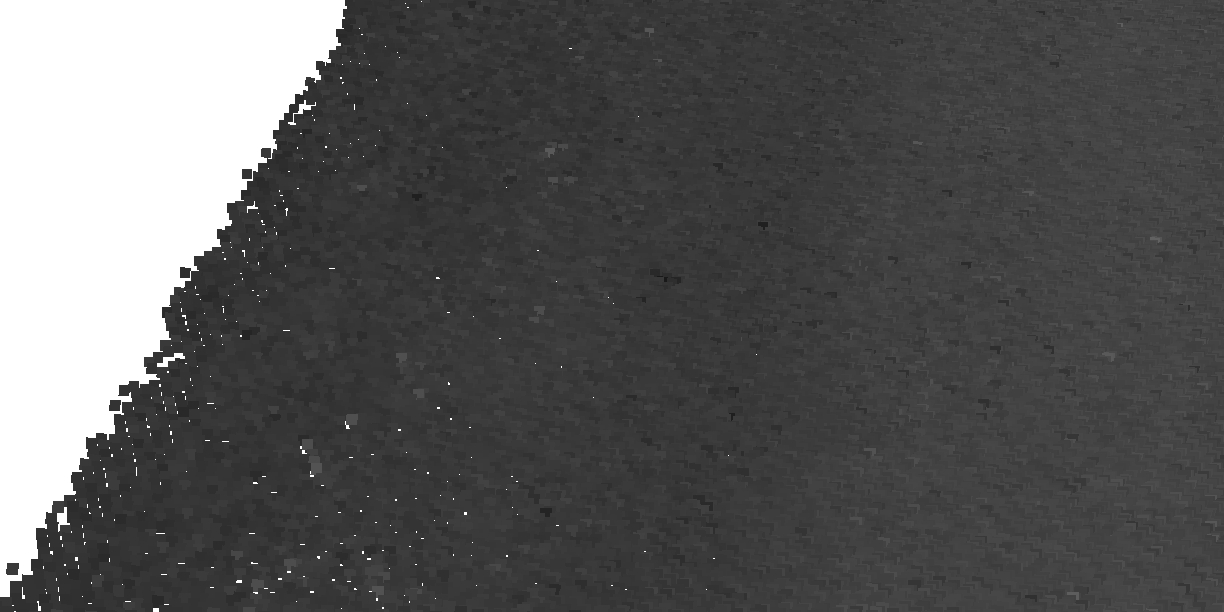
\includegraphics[width=0.32\textwidth]{graphics/class_undamaged}}
    \hfill
    \subcaptionbox{Schlagloch}{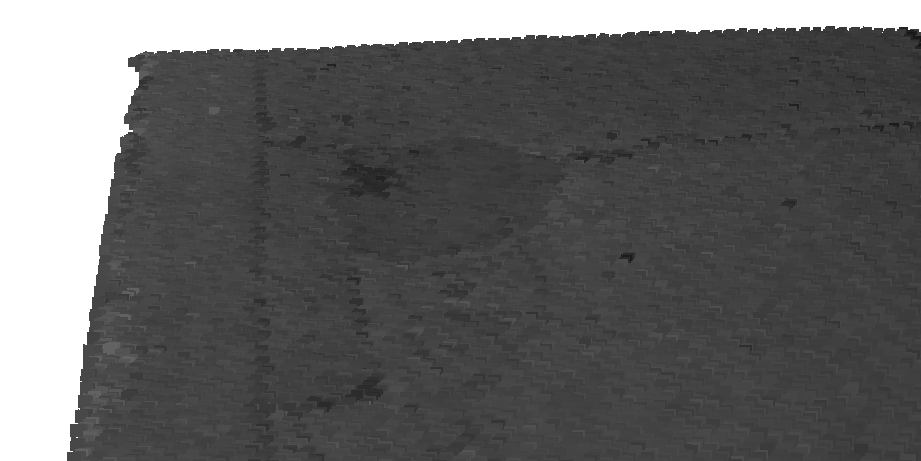
\includegraphics[width=0.32\textwidth]{graphics/class_pothole}}
    \hfill
    \subcaptionbox{Flickstelle}{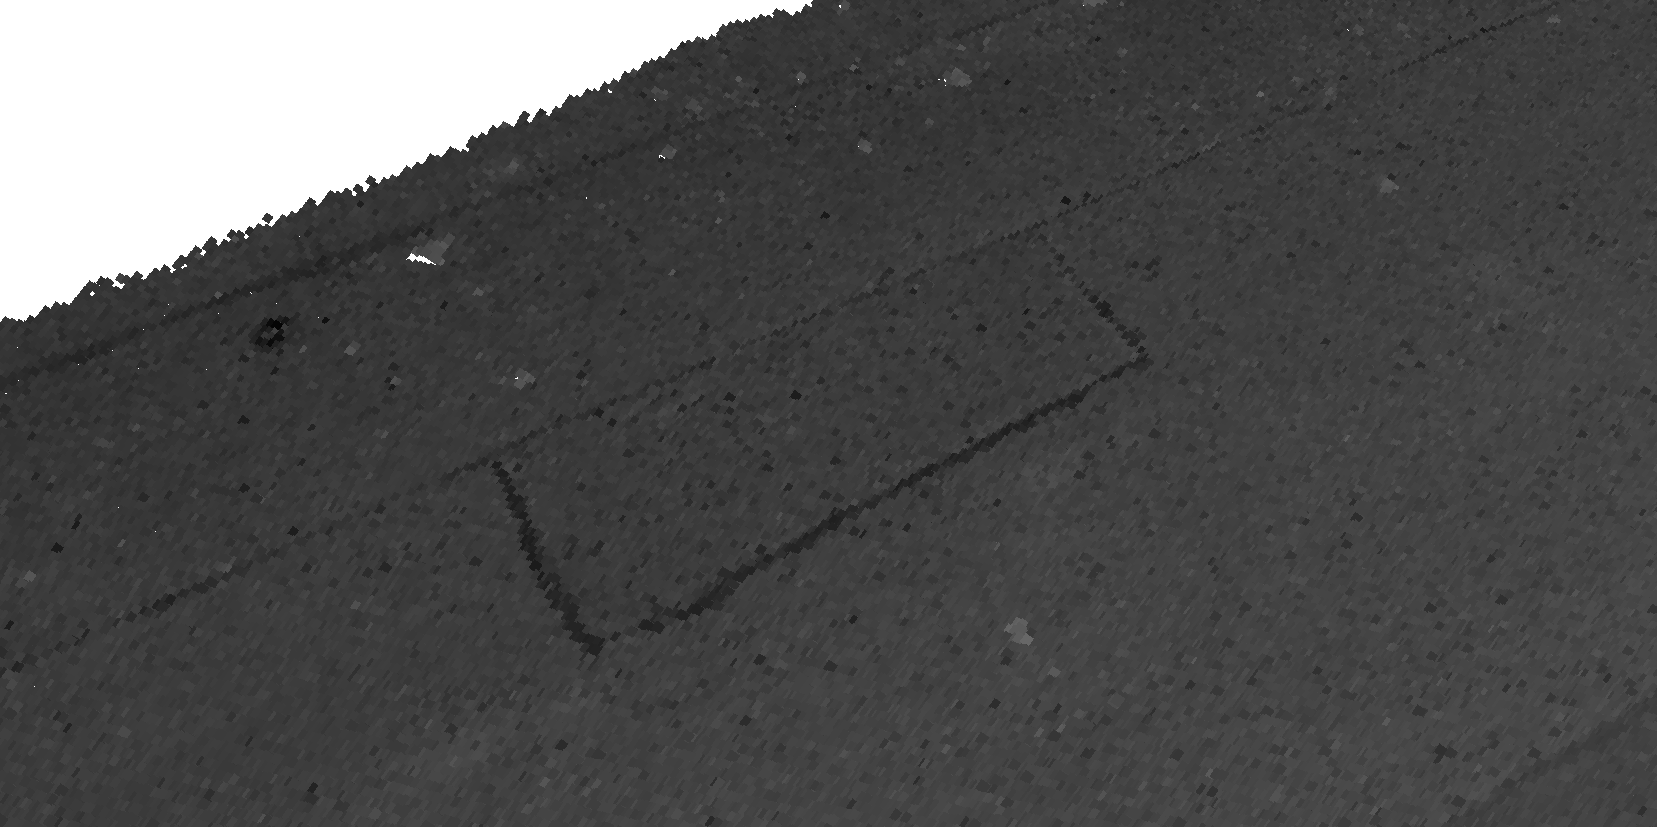
\includegraphics[width=0.32\textwidth]{graphics/class_flickstelle}}
    \par\medskip
    \subcaptionbox{Gullys unterschiedlicher Ausprägung}{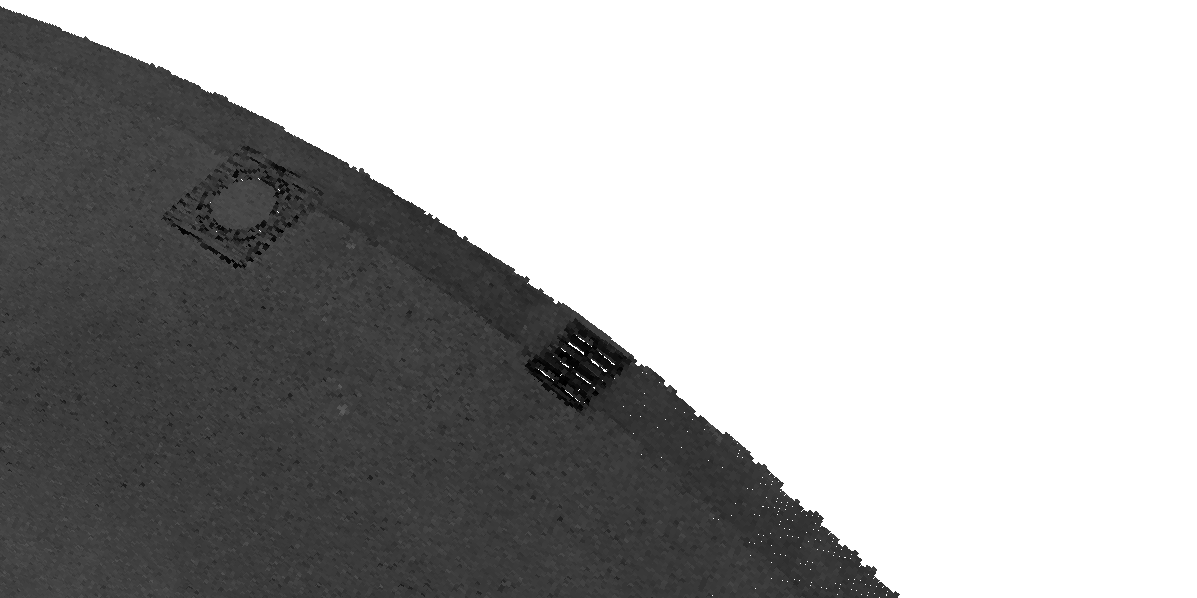
\includegraphics[width=0.32\textwidth]{graphics/class_gully}}
    \hfill
    \subcaptionbox{Ölfleck}{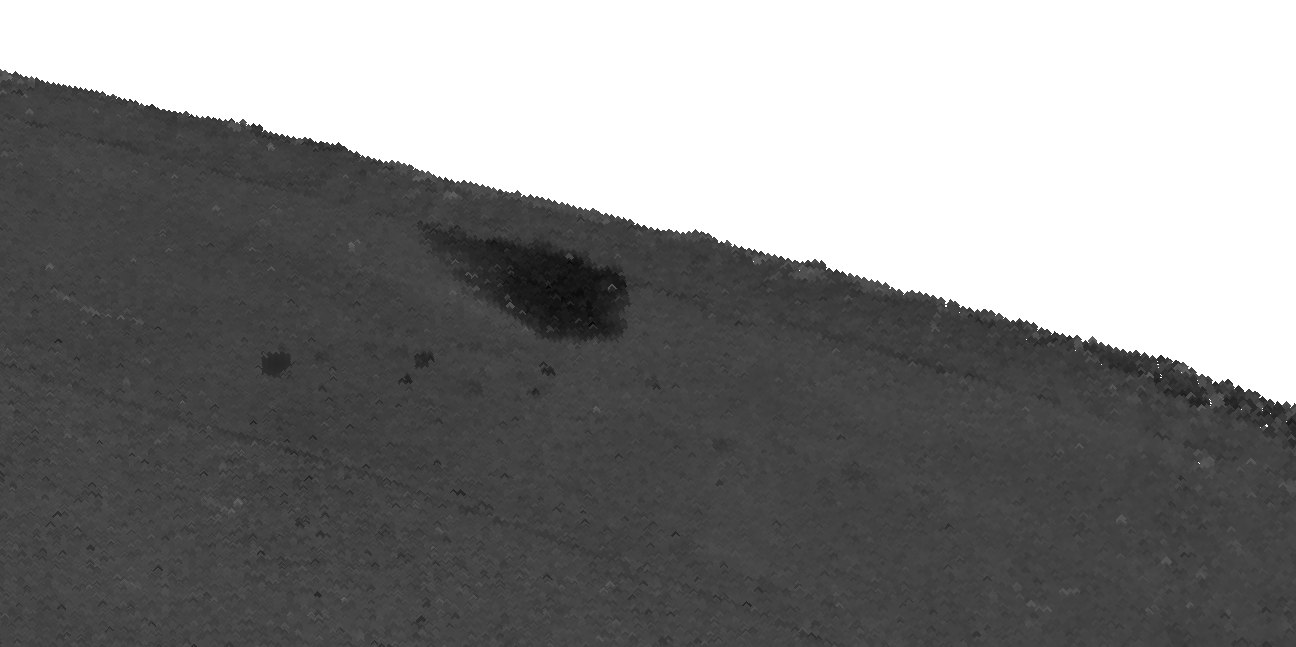
\includegraphics[width=0.32\textwidth]{graphics/class_spill}}
    \hfill
    \subcaptionbox{Fahrbahnmarkierung}{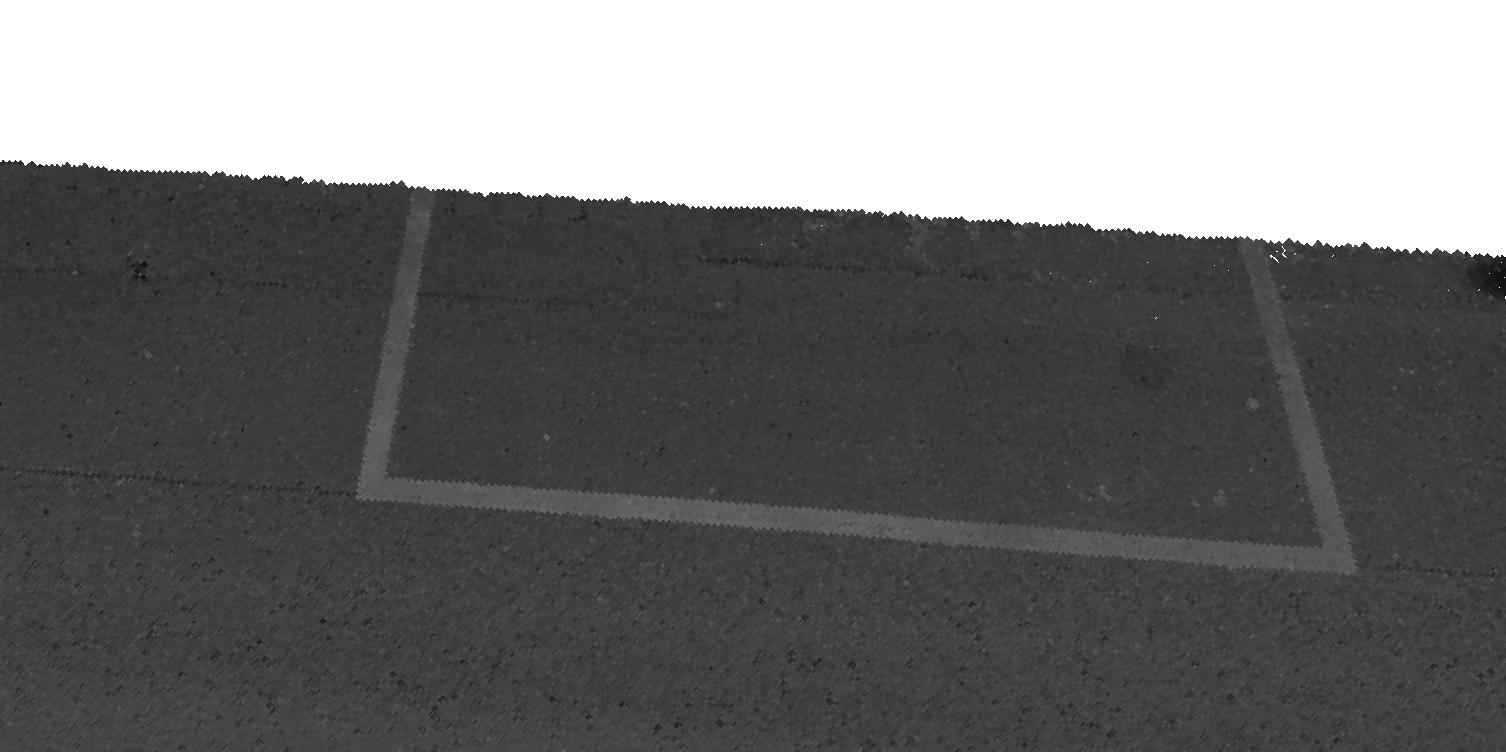
\includegraphics[width=0.32\textwidth]{graphics/class_road_marking}}
    \caption{Beispielhafte Bilder von zu erkennenden Objekten.}
    \label{fig:all_classes}
\end{figure}

Darunter fallen insbesondere merkliche Absenkungen wie Schlaglöcher oder Risse. Schlaglöcher zeichnen sich durch lokale Höhenunterschiede, welche von mehreren Millimetern bis hin zu einigen Zentimetern reichen können, sowie ihre meist eher rundliche Form aus. Durch den Aufriss der Fahrbahnoberfläche erscheinen sie außerdem dunkler als ihre unmittelbare Umgebung. \\
Auch Flickstellen bilden eine - im Vergleich zur gewöhnlichen Straße - auffällige Klasse: Sie werden angebracht, um beschädigte Straßenteile - wie zum Beispiel ein Schlagloch - zu überdecken und auf diese Weise ungefährlich zu machen. Charakterisiert werden sie durch ihre wegen der maschinellen Fertigung meist rechteckige Struktur sowie der im Vergleich zur Nachbarschaft oft dunkler erscheinenden Fugendichtmasse. Letztere kann durch Überquellen ebenfalls für marginale Höhenunterschiede an den Rändern sorgen. Flickstellen werden selbst bei Asphaltbelag auch zu den Schadensklassen gerechnet\footnote{https://itzeb.heller-ig.de/leitfaden/index.html?flickstellen\_\_\_fli\_efli\_afli.htm}. Straßenabschnitte mit einem hohen Anteil an Flickstellen sind entsprechend ein Hinweis auf nötige Reparaturen. \\
Gullys und Kanaldeckel kommen in vielen Ausprägungen bezüglich Größe und Form vor. Obwohl diese selbstverständlich begründet angelegt werden, zeichnen auch sie sich durch charakteristische Höhenunterschiede aus. Diese allgemeine Ähnlichkeit zu Schlaglöchern wirft die Frage nach ihrer Unterscheidbarkeit bezüglich ihrer Features auf, weshalb Gullys ebenfalls ein Ziel der Erkennung sind. Ein zuverlässiges Erkennen von Gullys kann außerdem, wie in Kapitel \ref{chap:uniqueness} erläutert wird, einen weiteren Vorteil bringen: Aufgrund ihrer beständigen Struktur können mehrere Punktwolken desselben Straßenabschnitts zueinander ausgerichtet werden. Damit könnte etwa die Veränderung des Straßenzustands in einem bestimmten Zeitraum dokumentiert werden. \\
Eine weitere Auffälligkeit sind besonders dunkle, unregelmäßige und teils sehr große Flecken. Ohne genaue Betrachtung vor Ort ist nicht zweifelsfrei auszumachen, worum es sich handelt: Bindemittelaustritte sind eine Alternative, aber auch Ölflecken sind möglich und (wegen der Nähe zu Parkplätzen in den genutzten Punktwolken) an dieser Stelle plausibel. Frische Ölflecken allerdings stellen augrund der geringen Griffigkeit eine große Rutschgefahr dar. Wegen dieser Option werden auch jene Stellen gesondert behandelt; der Einfachheit halber ist in der Arbeit folgend nur die Rede von Ölflecken. \\
Für den sicheren Straßenverkehr unerlässlich sind Fahrbahnmarkierungen. Durch ihre in der Materialzusammensetzung begründete Helligkeit sollen sie sich zu allen Tageszeiten und Wetterbedingungen stark abheben vom Rest der Fahrbahn und so Orientierung bieten. Von Interesse könnte hier insbesondere sein, ob und welche Markierungen sich stellenweise durch Verschleiß nicht mehr ihrem Zweck gemäß genug abheben und einer Auffrischung oder Erneuerung bedürfen. \\\\
Für die Bewertung des Straßenzustands spielen auch andere Elemente eine Rolle als unregelmäßige Schäden der Fahrbahnoberfläche wie Schlaglöcher. Dazu zählen zum Beispiel Spurrillen oder Unebenheiten der Straße auf Quer- und Längsseite um wenige Prozent, die unter Umständen über mehrere Meter gemessen werden. Andere Arbeiten wie \cite{Zhiqiang.etal-2019} und \cite{Famili.etal-2021} beziehen diese Mängel als Klassen in ihre \textit{Predictions} ein. \\
Die Erkennung solcher Schäden war kein Ziel dieser Arbeit, entweder aus Mangel an geeigneten und ausreichend vielen Daten oder, da andere Verfahren besser geeignet erscheinen. Für die Berechnung der Quer- wie Längsebenheit kommen beispielsweise 4$m$-Latten\footnote{http://www.vsvinrw.de/tl\_files/VSVI-NRW/Downloads/Seminarberichte/05\_2011/Oberflaecheneigenschaften\_und\_Strassenbautechnik.pdf} zum Einsatz, welche in regelmäßigen Abständen quer zur und längs der Straße gelegt werden. Anhand der Höhendifferenzen der Lattenenden können die gesuchten Werte mathematisch präzise ermittelt werden, ebenso andere Kenngrößen wie die Spurrinnentiefe oder fiktive Wassertiefe. Dieses Prinzip kann übertragen werden auf imaginäre Latten und Punktwolken der Straßen. Famili \textit{et al.} \cite{Famili.etal-2021} verfolgen ähnliche Vorgehensweisen über Funktionsgraphen von Querschnitten der Oberfläche. Solche geometrischen Verfahren sind bereits algorithmisch zu akkuraten Ergebnissen fähig. \\
Erst durch Kombination von Ansätzen, die sich auf solche verschiedenen Aspekte fokussieren, kann letztlich ein gesamtheitliches und aussagekräftiges Bild des Straßenzustands geschaffen werden. 

\section{Systemüberblick}

Beide Ansätze bauen auf ein System von bestehenden und abgeschlossenen Tools auf. Diese wurden teilweise ergänzt um nötige Erweiterungen für den \textit{Feature-Extraction}-Ansatz. \\\\
Das in dieser Arbeit bedeutsamste Werkzeug für die Prozessierung von Punktwolken ist das (in Kapitel \ref{chap:intro} kurz eingeführte) \texttt{PCTool}, einer in \texttt{C++} geschriebenen Anwendung. Dieses Framework bietet eine Vielzahl an Möglichkeiten zur effizienten Verarbeitung von Punktwolken. Die Grundbausteine sind sogenannte Knoten (\textit{Nodes}), die jeweils eine Operation zu Eingabe, Ausgabe oder Prozessierung implementieren. Dazu gehören zum Beispiel \textit{Reader} und \textit{Writer} von Punktwolken verschiedener Dateiformate. Auch die bereits erwähnten Funktionalitäten der Dichtereduktion und Bodenerkennung finden sich dort als separate Knoten wieder neben den für den eigenen Ansatz implementierten. Um die Knoten zu komplexeren Aktionen zu verknüpfen, können sie zu \textit{Pipelines} zusammengelegt werden. Ein Beispiel dazu findet sich in Abbildung \ref{fig:pcr_pipeline}, wo der beschriebene Ablauf des ersten Teils des eigenen Ansatzes zu sehen ist: vom Einlesen der Punktwolke, der Bodenerkennung und Straßenextraktion bis zum Ermitteln der Featurevektoren der einzelnen Punkte zur Schadenserkennung und Zurückschreiben der Punktwolke. (Anmerkung: Der einzelne \texttt{GroundDetector}-Knoten steht an dieser Stelle nur stellvertretend für die im Projekt genutzte elaboriertere Bodenerkennung, siehe \cite{Mattes-2021}.) Auf die Hintergründe der \texttt{StreetExtractor}- und \texttt{PavementDistressDetector}-Knoten wird in nachfolgenden Kapiteln näher eingegangen. \\\\

\begin{figure}[!ht]
    \centering
    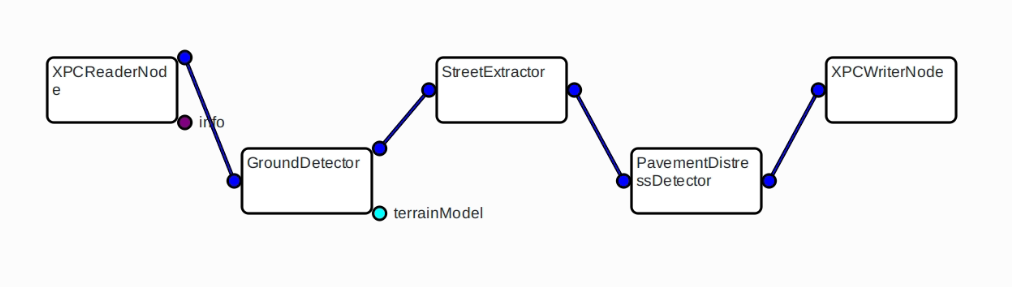
\includegraphics[width=0.95\textwidth]{graphics/pcr_pipeline}
    \caption{Die eingesetzte Pipeline im PCTool für die Featureberechnung.}
    \label{fig:pcr_pipeline}
\end{figure}

Der zweite Schritt des \textit{Feature-Extraction}-Ansatzes, den \textit{Predictions} der einzelnen Punktklassen anhand der Featurevektoren, findet sich in einer Reihe von Python-Skripten. Diese sind Teil des im Projekt entstandenen sogenannten \textit{Modelzoo}, der eine Menge von Funktionalitäten des maschinellen Lernens für die Webplattform \citep{Schilling-2021} bietet. Unter anderem ist dort auch die Klassifizierung von Punktwolken anhand ihres sogenannten \textit{Point Cloud Fingerprints} gelegen, einer Art globaler und kompakter Repräsentation \citep{Kirsten-2021}. Für den eigenen Ansatz werden vor allem Schnittstellen zum Trainieren und Testen von Modellen für die \textit{Predictions} obiger Klassen bereitgestellt, siehe Kaptiel \ref{chap:prediction}. \\
Der Grund für die Trennung der Featureberechnung und \textit{Prediction} in zwei Teilsysteme, was einen verhältnismäßig hohen Zusatzaufwand bedeutet durch Übertragung und Zwischenspeicherung der Featurevektoren, liegt in der Handhabbarkeit. Python ist im Bereich des maschinellen Lernens eine etablierte Wahl und bietet insbesondere einfach zu nutzende Schnittstellen. Langfristig ist daher für eine Effizienzsteigerung die Integration des \textit{Prediction}-Teilsystems in \texttt{C++} bzw. im Speziellen das \texttt{PCTool} anzustreben. \\\\
Mit Hilfe des \texttt{PCNN}-Frameworks, in Kapitel \ref{chap:intro} eingeführt, wurde der \textit{Deep-Learning}-Ansatz getestet. Näheres zur Architektur und Bedienung findet sich in Kapitel \ref{chap:deepl}. Etwaige Bilder von Punktwolken wurden angefertigt mit dem lehrstuhleigenen \texttt{PCViewer}, welcher eine Vielzahl an Möglichkeiten zur Visualisierung der einzelnen Punkte bietet. \\
Das letzte im Zuge dieser Arbeit genutzte Programm ist das \texttt{TrainingTool}, das der Annotation der Klassen pro Punkt dient. Um sich eine Grundlage für die Experimente dieser Arbeit zu schaffen und mangels geeigneter vorhandener Datensätze, wurden damit die Schlaglöcher, Gullys und alle weiteren erwähnten Klassen manuell nach bestem Wissen und Gewissen markiert. Insbesondere wegen der teils feinen Objekte sowie der begrenzten Auflösung der Punktwolken ist damit aber immer eine Unsicherheit behaftet. Gerade bezüglich der Grenzen von Flickstellen und Ränder von Schlaglöchern ist diese Einschränkung in der qualitativen und quantitativen Analyse der \textit{Predictions} zu berücksichtigen, die sich in Kapitel \ref{chap:eval} findet.